\subsubsection{bringit::client::view::list::input::InputListInfoView}

\label{bringit::client::view::list::input::InputListInfoView}
\begin{figure}[H]
	\centering
	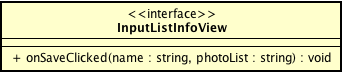
\includegraphics[scale=0.5]{Sezioni/SottosezioniST/img/app/InputListInfoView.png}
	\caption{bringit::client::view::list::input::InputListInfoView}
\end{figure}

\begin{itemize}
\item \textbf{Descrizione}: La view relativa alla parte grafica di inserimento dei dati di una lista.
\item \textbf{Utilizzo}: L'interfaccia viene utilizzata per disaccoppiare presenter e implementazione della classe e per visualizzare i dati che gli vengono passati dal presenter.
\item \textbf{Attributi}: 
\item \textbf{Metodi}:
	\begin{itemize}
	\item \textit{public onSaveClicked():void}\\
	Questo metodo crea una lista con i dati inseriti, emettendo un evento \textit{'emitSaveEvent'}.
	\end{itemize}
\end{itemize} 

\subsubsection{bringit::client::view::list::input::view::InputListInfoViewImpl}

\label{bringit::client::view::list::input::view::InputListInfoViewImpl}
\begin{figure}[H]
	\centering
	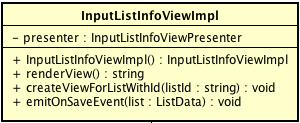
\includegraphics[scale=0.5]{Sezioni/SottosezioniST/img/app/InputListInfoViewImpl.png}
	\caption{bringit::client::view::list::input::view::InputListInfoViewImpl}
\end{figure}

\begin{itemize}
\item \textbf{Descrizione}: Questa classe rappresenta la classe concreta di inserimento dei dati di una lista.
\item \textbf{Utilizzo}: Implementando i metodi di InputListInfoView questa classe viene utilizzata al momento dell'inserimento dei dati di una lista bringit da Rocket.Chat.
\item \textbf{Attributi}: 
\begin{itemize}
	\item \textit{private presenter:InputListInfoViewPresenter}\\
	Il presenter relativo all'inserimento dei dati della lista.
	\item \textit{private saveEvent:SaveEventEmitter}\\
	Il riferimento all'oggetto responsabile dell'emissione degli eventi di salvataggio su database.
\end{itemize}
\item \textbf{Metodi}:
	\begin{itemize}
	\item \textit{public InputListInfoViewImpl():InputListInfoViewImpl}\\
	Il costruttore di InputListInfoViewImpl.
	\item \textit{public onSaveClicked(name:string,photoList:string):void}\\
	Questo metodo crea una lista con i dati inseriti, emettendo un evento \textit{'emitSaveEvent'}.
					\\ \textbf{Parametri}: \begin{itemize}
			\item \textit{name:string}\\
			Il nome della lista che si sta per creare.
			\item \textit{photoList:string}\\
			Il percorso dell'immagine della lista.
					\end{itemize} 
	\end{itemize}
\end{itemize} 

\subsubsection{bringit::client::view::list::input::presenter::InputListInfoViewPresenter}

\label{bringit::client::view::list::input::presenter::InputListInfoViewPresenter}
\begin{figure}[H]
	\centering
	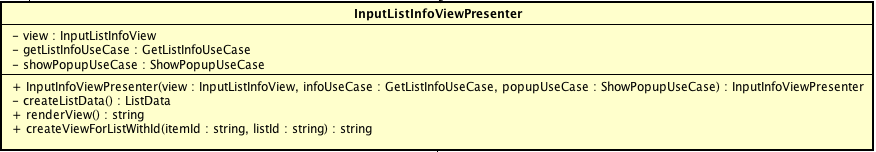
\includegraphics[scale=0.5]{Sezioni/SottosezioniST/img/app/InputListInfoViewPresenter.png}
	\caption{bringit::client::view::list::input::preseter::InputListInfoViewPresenter}
\end{figure}

\begin{itemize}
\item \textbf{Descrizione}: Questa classe rappresenta il presenter per la classe di eliminazione della lista bringit.
\item \textbf{Utilizzo}: Il presenter fa da tramite tra l'implementazione e la view, formattando i dati che verranno visualizzati nella view e manipolando gli input dell'utente per eseguire le operazioni logiche predisposte.
\item \textbf{Attributi}: 
	\begin{itemize}
	\item \textit{private chat:ChatSource}\\
	Il riferimento alla classe necessaria per interfacciarsi a Rocket.Chat.
	\item \textit{private view:InputListInfoView}\\
	La view necessaria al presenter.
	\item \textit{private popup:ShowPopupUseCase}\\
	Il riferimento all'oggetto necessario per il display di popup in Rocket.Chat.
	\end{itemize}
\item \textbf{Metodi}:
	\begin{itemize}
	\item \textit{public InputListInfoViewPresenter(view:InputListInfoView):InputListInfoViewPresenter}\\
	Il costruttore di InputListInfoViewPresenter.
					\\ \textbf{Parametri}: \begin{itemize}
			\item \textit{view:InputListInfoView}\\
			La view necessaria al presenter.
					\end{itemize} 
	\item \textit{public createListData(name:string,image:string):ListData}\\
	Questo metodo crea una lista con i dati inseriti, e la ritorna.
					\\ \textbf{Parametri}: \begin{itemize}
			\item \textit{name:string}\\
			Il nome della lista che si sta per creare.
			\item \textit{image:string}\\
			Il percorso dell'immagine della lista.
					\end{itemize} 
	\end{itemize}
\end{itemize} 
 
